%!TEX root = ../paper.tex

\begin{table}[t]
\begin{center}
\small
\begin{tabular}{| p{2cm} | p{1cm} | p{1cm} | p{1cm} | c |}
\hline
Technology & Q1 &  Median & Q3 & Distribution  \\ 
\hline
Location Tracking & 10.0 & 10.0 & 20.0 & 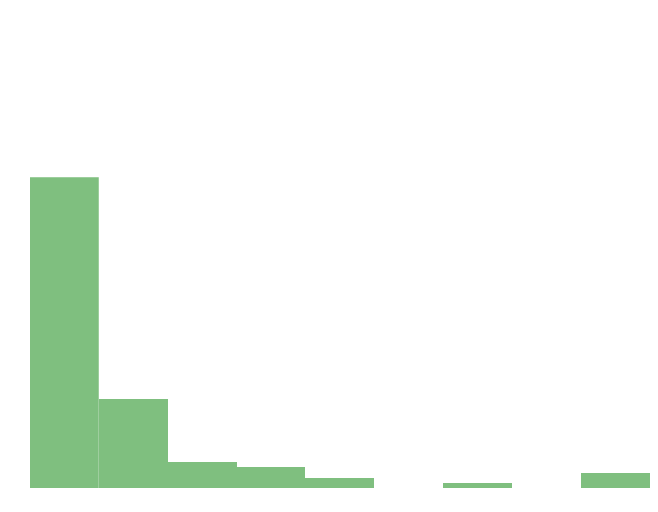
\includegraphics[width = 2cm, height = 0.5cm]{tex-inputs/table-images/locationtrackingrisk} \\ 
Speech To Text & 10.0 & 10.0 & 10.0 & 
\includegraphics[width = 2cm, height = 0.5cm]{tex-inputs/table-images/speechtotextrisk} \\ 
Discreet Microphone & 10.0 & 10.0 & 20.0 & 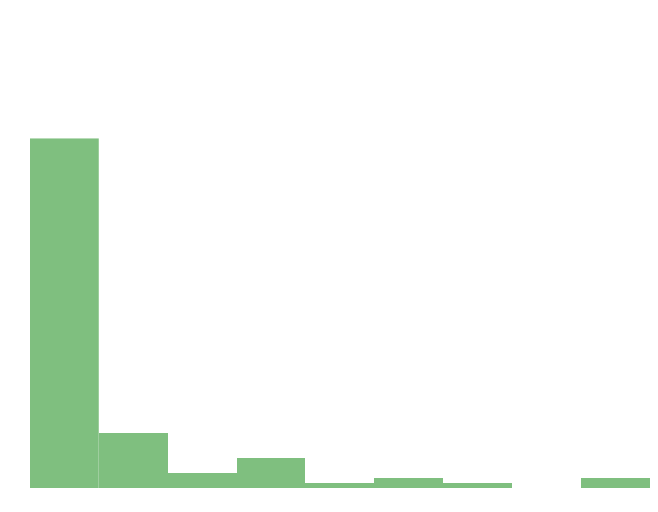
\includegraphics[width = 2cm, height = 0.5cm]{tex-inputs/table-images/discreetmicrophonerisk} \\ 
Smartwatches & 10.0 & 10.0 & 10.0 & 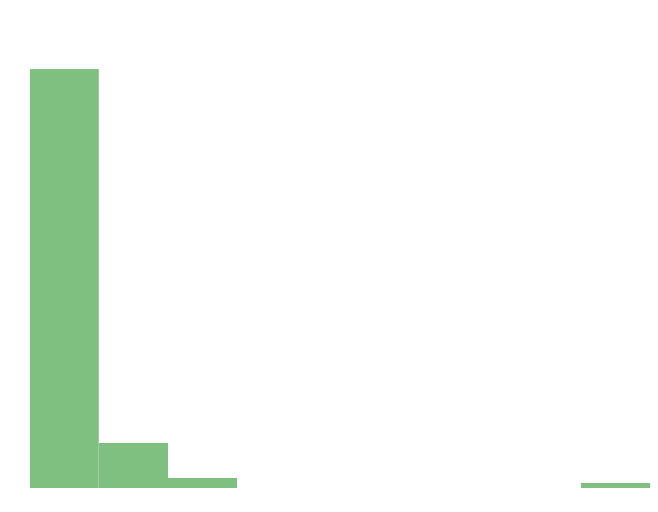
\includegraphics[width = 2cm, height = 0.5cm]{tex-inputs/table-images/smartwatchesrisk} \\ 
Language Detection & 10.0 & 10.0 & 10.0 & 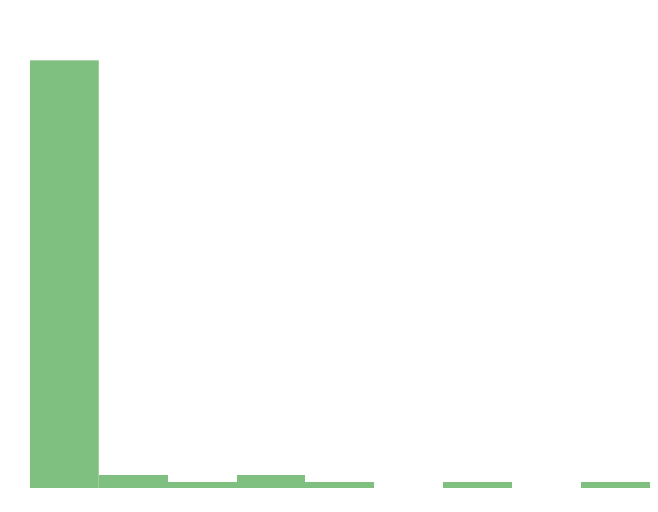
\includegraphics[width = 2cm, height = 0.5cm]{tex-inputs/table-images/languagedetectionrisk} \\ 
Laptops & 10.0 & 10.0 & 15.0 & 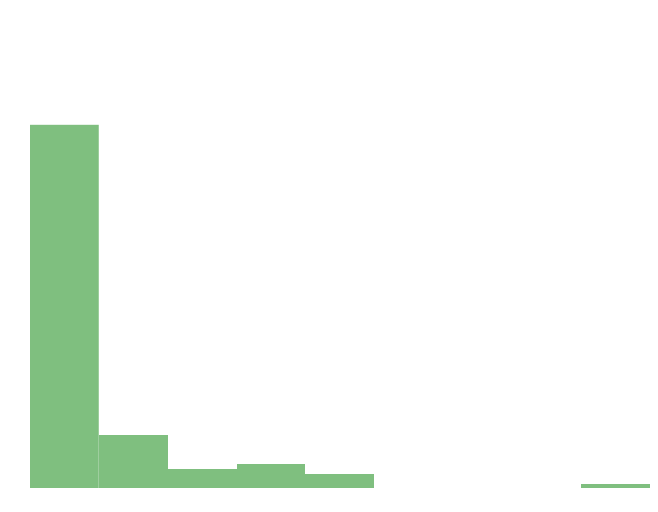
\includegraphics[width = 2cm, height = 0.5cm]{tex-inputs/table-images/laptopsrisk} \\ 
Smartphones & 10.0 & 10.0 & 20.0 & 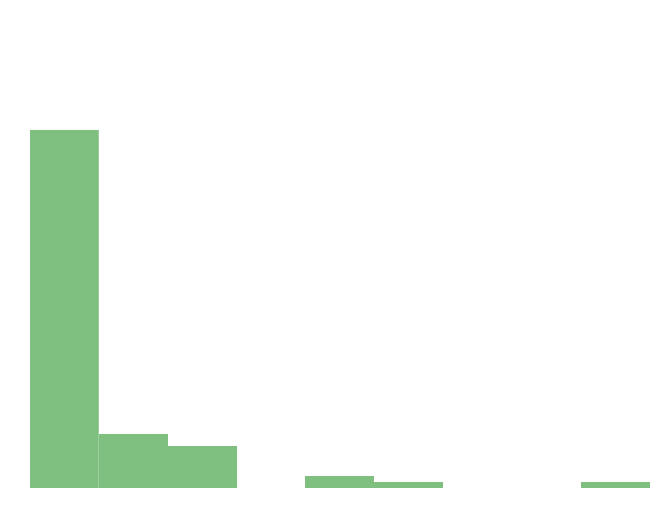
\includegraphics[width = 2cm, height = 0.5cm]{tex-inputs/table-images/smartphonesrisk} \\ 
Google Glass & 10.0 & 10.0 & 20.0 & 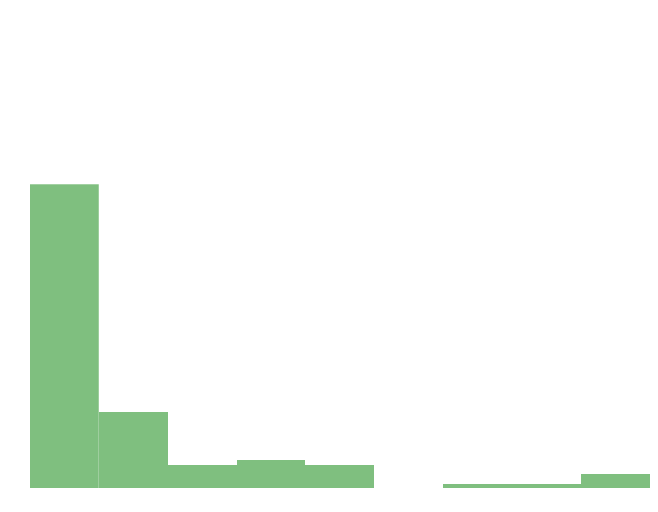
\includegraphics[width = 2cm, height = 0.5cm]{tex-inputs/table-images/googleglassrisk} \\ 
Cubetastic & 10.0 & 10.0 & 30.0 & 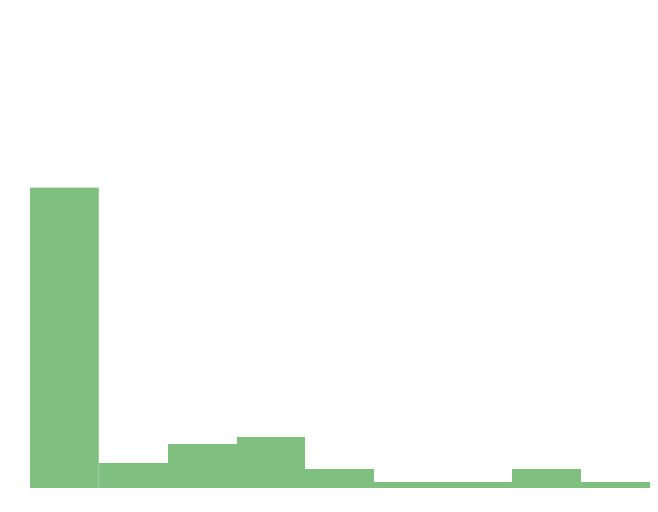
\includegraphics[width = 2cm, height = 0.5cm]{tex-inputs/table-images/cubetasticrisk} \\ 
Gender Detection & 10.0 & 10.0 & 13.5 & 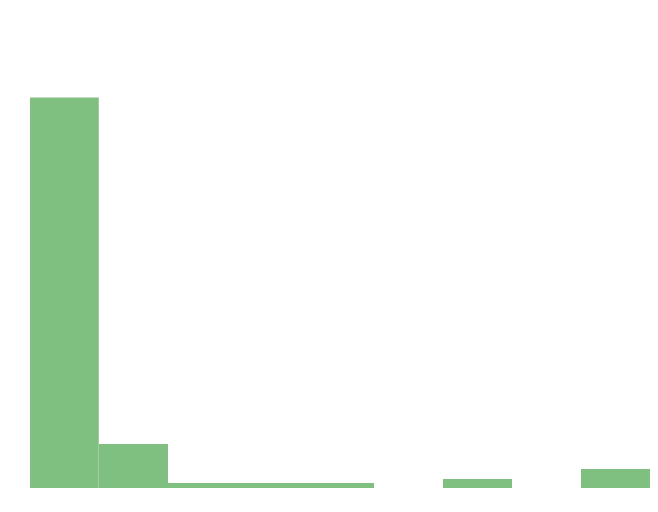
\includegraphics[width = 2cm, height = 0.5cm]{tex-inputs/table-images/genderdetectionrisk} \\ 
Voice Recognition & 10.0 & 10.0 & 15.0 & 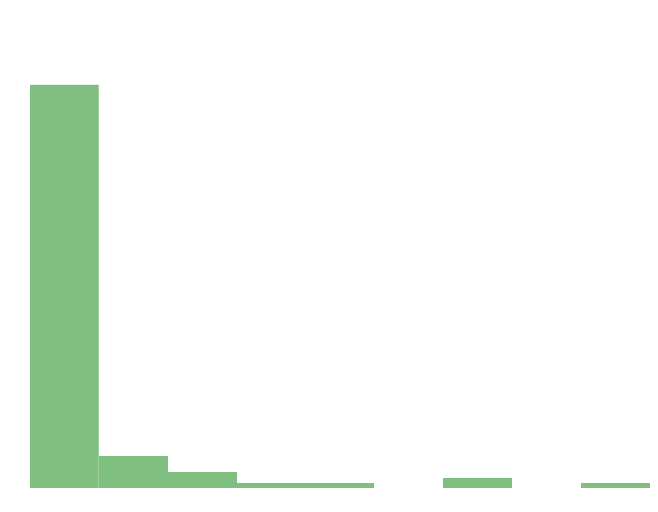
\includegraphics[width = 2cm, height = 0.5cm]{tex-inputs/table-images/voicerecognitionrisk} \\ 
Voice Based Emotion Detection & 10.0 & 10.0 & 15.0 & 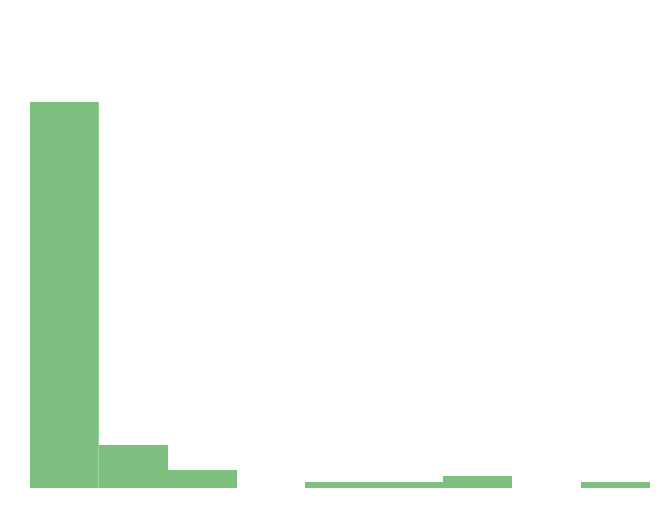
\includegraphics[width = 2cm, height = 0.5cm]{tex-inputs/table-images/voicebasedemotiondetectionrisk} \\ 
Fitness Trackers & 10.0 & 10.0 & 10.0 & 
\includegraphics[width = 2cm, height = 0.5cm]{tex-inputs/table-images/fitnesstrackersrisk} \\ 
Age Detection & 10.0 & 10.0 & 15.0 & 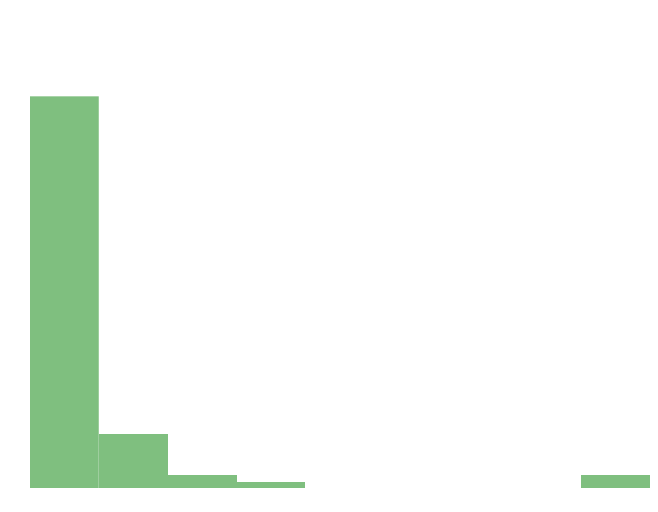
\includegraphics[width = 2cm, height = 0.5cm]{tex-inputs/table-images/agedetectionrisk} \\ 
Facial Detection & 10.0 & 10.0 & 25.0 & 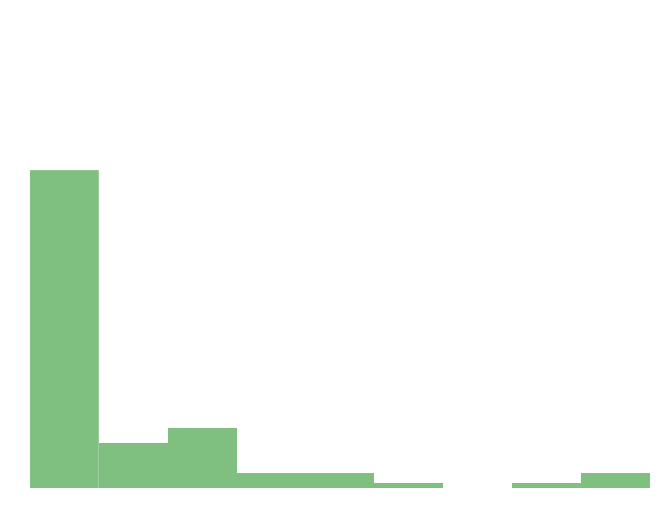
\includegraphics[width = 2cm, height = 0.5cm]{tex-inputs/table-images/facialdetectionrisk} \\ 
Email & 10.0 & 10.0 & 18.0 & 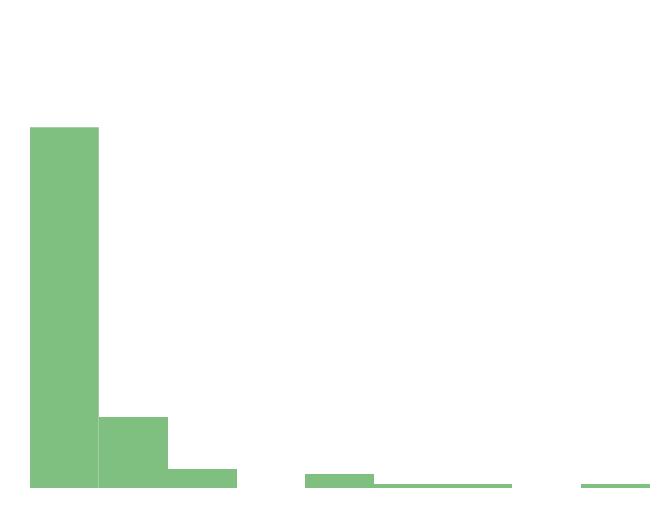
\includegraphics[width = 2cm, height = 0.5cm]{tex-inputs/table-images/emailrisk} \\ 
Heart Rate Detection & 10.0 & 10.0 & 10.0 & 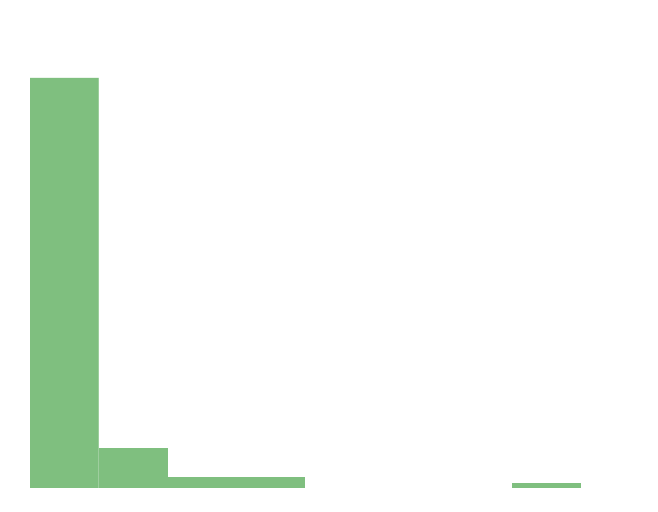
\includegraphics[width = 2cm, height = 0.5cm]{tex-inputs/table-images/heartratedetectionrisk} \\ 
Discreet Video Camera & 12.0 & 10.0 & 30.0 & 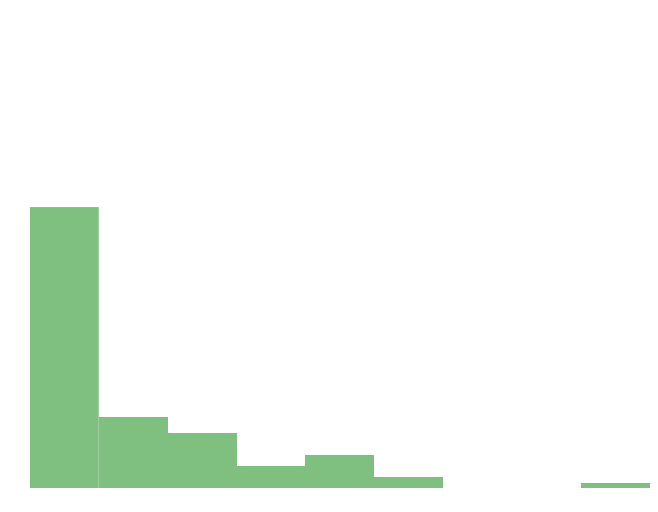
\includegraphics[width = 2cm, height = 0.5cm]{tex-inputs/table-images/discreetvideocamerarisk} \\ 
Internet & 15.0 & 10.0 & 31.0 & 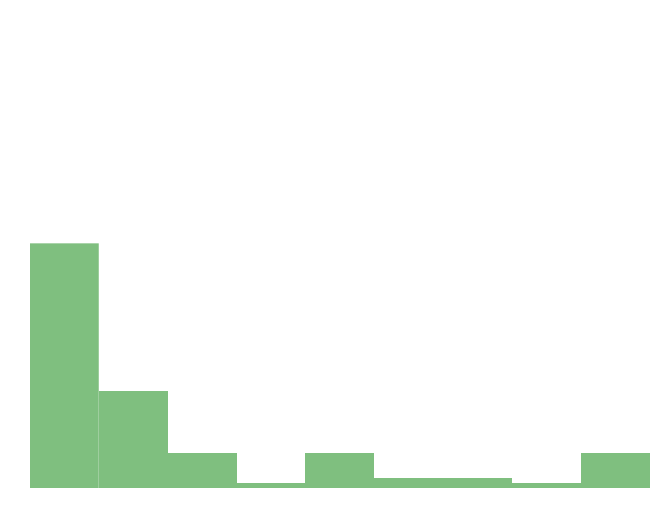
\includegraphics[width = 2cm, height = 0.5cm]{tex-inputs/table-images/internetrisk} \\ 
Facial Recognition & 17.0 & 10.0 & 30.0 & 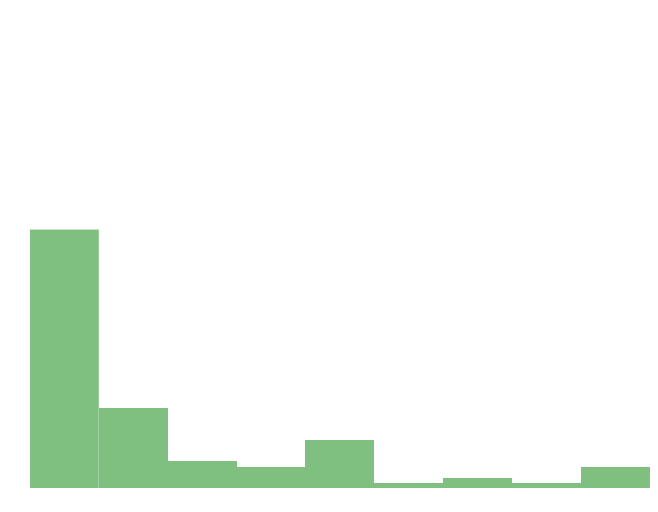
\includegraphics[width = 2cm, height = 0.5cm]{tex-inputs/table-images/facialrecognitionrisk} \\ 
Lawnmower & 20.0 & 12.0 & 30.0 & 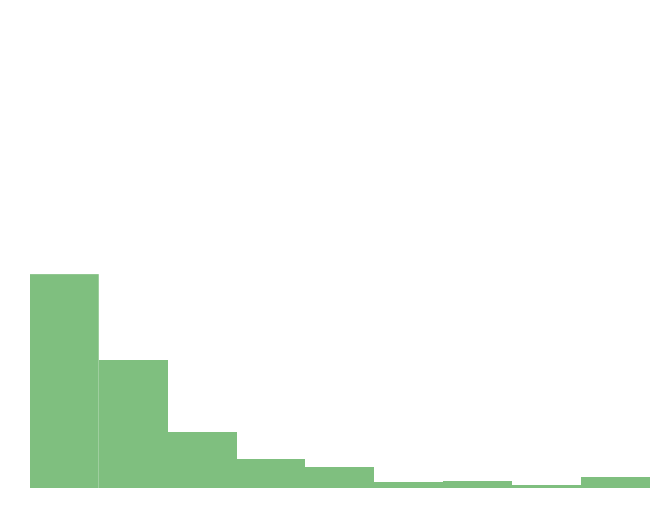
\includegraphics[width = 2cm, height = 0.5cm]{tex-inputs/table-images/LawnmowerRisk} \\ 
Electricity & 25.0 & 15.0 & 40.0 & 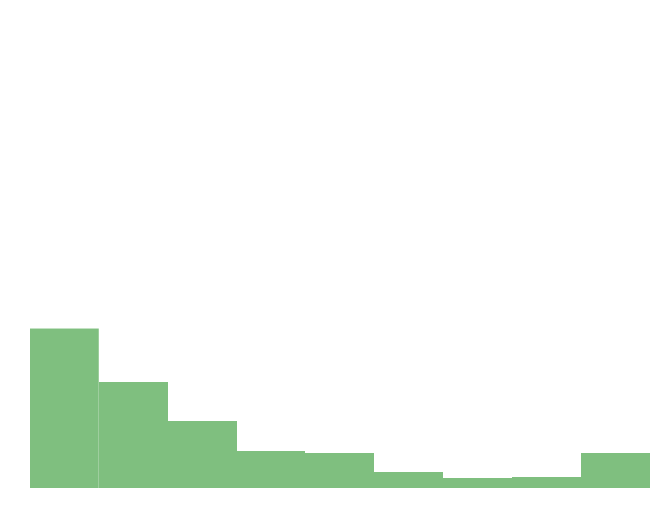
\includegraphics[width = 2cm, height = 0.5cm]{tex-inputs/table-images/ElectricityRisk} \\ 
Motorcycle & 45.0 & 27.0 & 70.0 & 
\includegraphics[width = 2cm, height = 0.5cm]{tex-inputs/table-images/MotorcycleRisk} \\ 
Handgun & 60.0 & 40.0 & 100.0 & 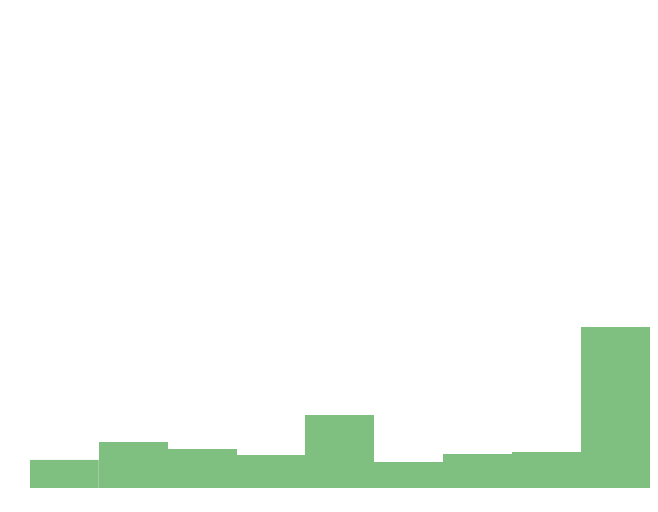
\includegraphics[width = 2cm, height = 0.5cm]{tex-inputs/table-images/HandgunRisk} \\ 
\hline
\end{tabular}
\caption{The 10 most and least upsetting data types, across all recipients.}
\label{top10}
\end{center}
\end{table}
